\chapter{粮食安全问题}
\label{chapter:Food security problem}

习近平总书记指出,粮食安全是“国之大者”,耕地是粮食生产的命根子,确保18亿亩耕地红线决不突破。

在全球化的背景下,粮食安全问题成为国际社会关注的焦点。作为世界上人口数量位居前列的国家,中国在粮食安全方面的表现不仅关乎其经济发展和社会稳定,还对维护全球粮食安全体系发挥着关键作用。而农村地区,作为粮食生产的主要基地,承担着维护国家粮食安全的重要责任。

\section{农作物播种面积}

粮食安全的基础在很大程度上依赖于稳定且充足的播种面积。播种面积不仅直接影响到粮食的总产量,也关系到农业的可持续性和对环境变化的适应能力。本文收集到了1990-2022年的农作物总播种面积。为直观分析这一时期内播种面积的波动和趋势,本文计算出播种面积的平均值,并利用玫瑰图展示各年度播种面积相对于平均值的变化,如下图所示:
\begin{figure}[H]
    \centering
    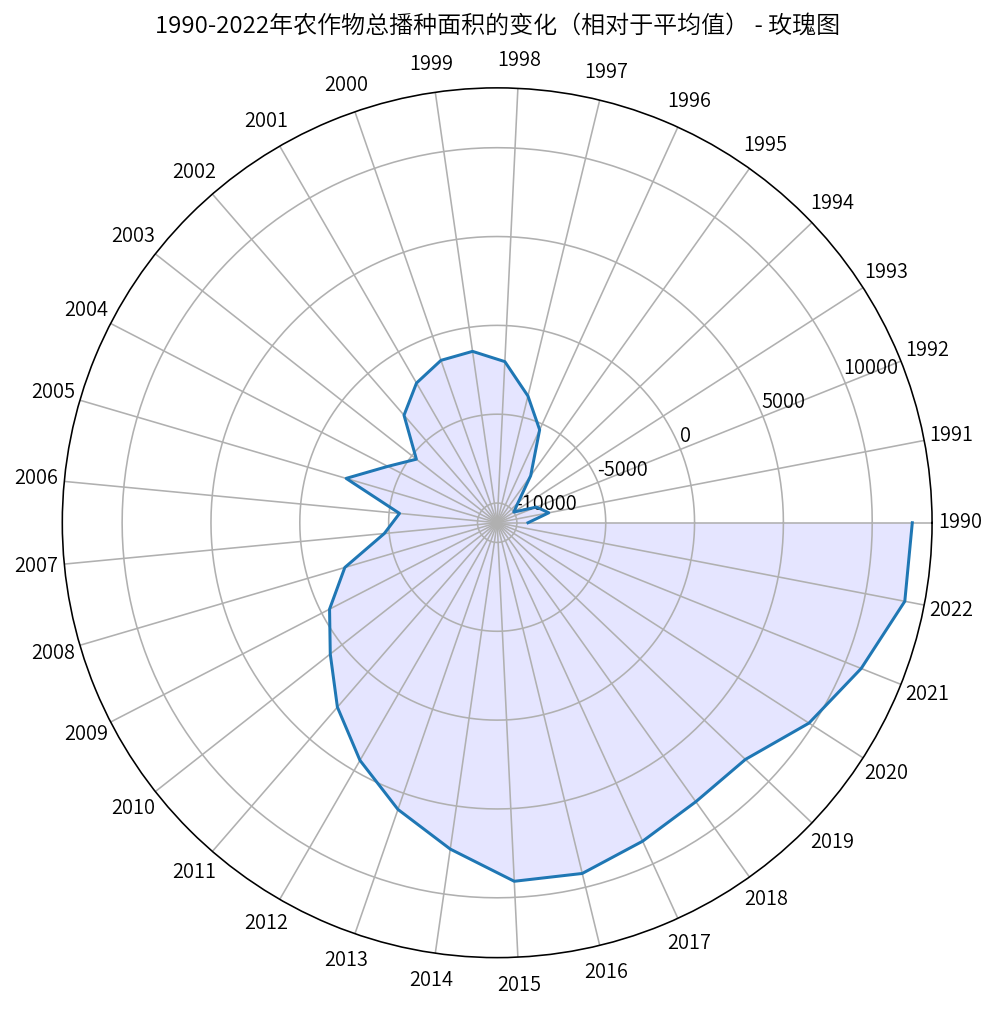
\includegraphics[width=0.5\linewidth]{figures/5.png}
    \caption{1990-2022年农作物总播种面积变化图}
    \label{fig:Total_sown_area}
\end{figure}

从图中可以看出,大多数花瓣沿着径向向外扩展,这表明随着时间的推进,播种面积呈现出增长趋势。这种增长通常指示了农业用地的扩张,对粮食安全来说是一个积极的信号,因为这意味着有潜力生产更多的粮食来满足日益增长的人口需求。同时,这样的增长也应当与生态和可持续发展原则相协调。

\section{主要粮食产量}

通过阅读农业农村部门文件农办科〔2023〕15号以及其他相关文献,可以了解到中国的农业生产主要集中在小麦、稻谷、大豆和玉米等主食农作物上。这些作物的生产状况对我国的粮食安全至关重要。

同样,本文收集了1990年到2022年间的粮食产量数据。为了更清晰地展示近年来的发展趋势,本文截取了2005年至2022年间的数据绘制了折线图,如下图所示:

\begin{figure}[H]
    \centering    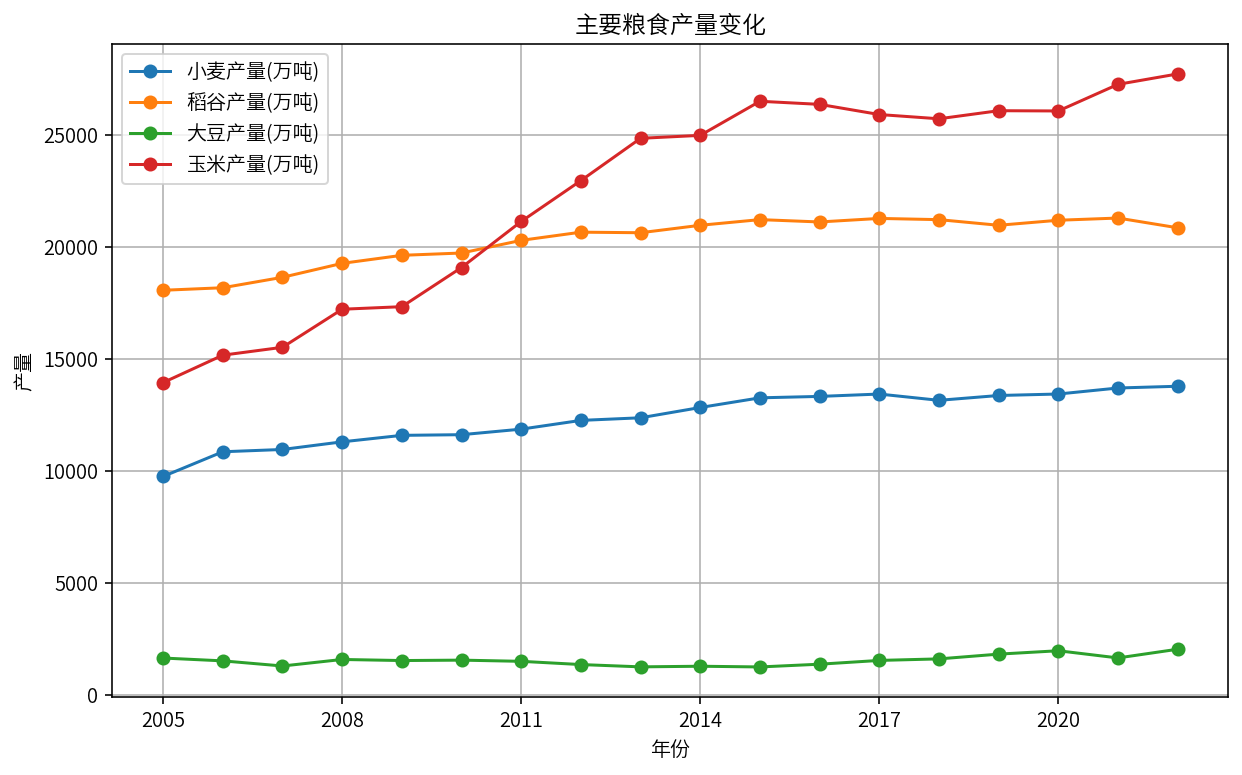
\includegraphics[width=0.9 \linewidth]{figures/8.png}
    \caption{主要粮食产量变化}   \label{fig:Changes_grain_production}
\end{figure}

此折线图清晰地呈现了自2005年以来中国主要粮食作物的产量变化。显著的是,水稻、小麦和玉米三者的产量逐年攀升,这一趋势不仅标志着农业技术进步和生产效率的提高,也反映了中国乡村振兴策略成功增强了农村地区的农业生产能力。鉴于这些作物在中国饮食中占据基础性地位,它们产量的增加直接增强了国家粮食安全保障。

此外,在十四届全国人民代表大会第二次会议上,国务院提出了我国粮食库存消费比的最新数据,显示我国的粮食库存消费比远高于联合国粮农组织建议的17\%-18\%的国际安全水平。这一数据不仅展示了我国在粮食安全领域所取得的显著成就,也反映了国家对于保障粮食安全的高度重视和扎实努力。